\documentclass[journal]{IEEEtran}
\usepackage{graphicx,mathtools,epstopdf,epsfig,pdflscape,hyperref}
\usepackage[T1]{fontenc}
\DeclarePairedDelimiter{\floor}{\lfloor}{\rfloor}

\begin{document}

\title{EsgalDNS: Tor-powered Consensus-based Distributed DNS for Tor Hidden Services\\ \Large Noisy DNS from Quiet Places}
\author{Jesse Victors \\ October 2014}

\maketitle

\section{Abstract}

Tor is a second-generation onion routing system that aims to provide anonymity, privacy, and Internet censorship resistance to its users. In recent years it has grown significantly in response to revelations of national and global electronic surveillance, and remains one of the most popular and secure anonymity network in use today. While it used most often for accessing the clearnet, Tor also supports anonymous websites within its network. Decentralized and secure, the domain names for these services are tied to public key infrastructure but are challenged by their long and technical addresses. In response to this difficulty, I propose a decentralized DNS system that is embedded in the Tor network. This system provides a securely unique mapping between human-readable names and traditional Tor hidden service addresses. This paper serves as a brief overview and initial rough draft of this proposal.

\section{Background}

\subsection{Overview of Tor}

Tor has been recognized by the NSA as the "the king of high secure, low latency Internet anonymity". The term Tor refers both to the client-side multiplexing software and to the worldwide volunteer-run network of over six thousand nodes. The Tor software provides an anonymity and privacy layer by relaying all end-user TCP traffic through a series of relays on the Tor network. Typically this route consists of a carefully-constructed three-hop path known as a \textit{circuit}, which changes over time. These nodes in the circuit are commonly referred to as \textit{guard node}, \textit{middle relay}, and the \textit{exit node}, respectively. Only the first node is exposed to the origin of TCP traffic into Tor, and only the exit node can see the destination of traffic out of Tor. The middle router, which passes encrypted traffic between the two, is unaware of either. The client negotiates a separate TLS connection with each node at a time, and traffic through the circuit is decrypted one layer at a time. This makes Tor much more resilient to traffic analysis in comparison to a VPN or to a direct TLS connection.

\begin{figure}[htbp]
	\centering
	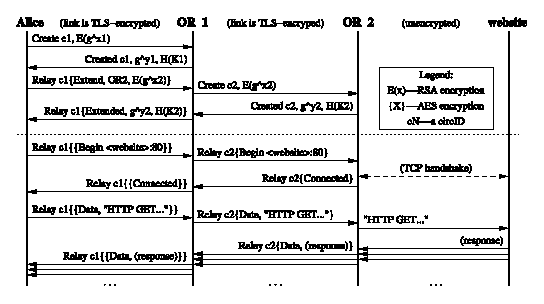
\includegraphics[width=0.5\textwidth]{../images/onion_layers.eps}
	\caption{Construction of a Tor circuit and a torified web GET request}
	\label{fig:figure3}
\end{figure}

The Tor network is managed by nine authority nodes. All nodes in the Tor network periodically send status reports to these authorities. The authority nodes in turn broadcast to the Tor network a digitally signed list containing IPs, ports, public keys, status, capabilities, and other information about all nodes on the network. Thus the Tor network is a interconnected graph.

\subsection{Tor Hidden Services}

While Tor is most frequently used to anonymously or privately access the Internet, it also supports anonymous services such as websites, marketplaces, and chatrooms. Tor hidden services are a part of the Dark Web and cannot be normally contacted outside of Tor. They allow a client, Alice, and a hidden service, Bob, to communicate with bidirectionally anonymously. Tor does not contain a DNS system for its hidden services; instead, services are accessed by hexadecimal identifiers. Every hidden service contains a public and private RSA key pair and its domain name is a truncated hash of its public key with the top-level domain (TLD) as .onion.

The hidden service Bob enables communication by first building Tor circuits to several random relays. He then tells them his public key, $ B_{K} $, enabling them to act as \textit{introduction points} for his services. He digitally signs a list of these introduction points and uploads the list to a distributed hash table inside the Tor network. A client Alice with Bob's hexadecimal domain name can initiates contact by first querying this hashtable for $ B_{K} $ and Bob's introduction points. She can verify that the domain name she queried is a truncated hash of $ B_{K} $, which allows her to prove Bob's authenticity. Secondly, she builds a circuit to random relay, $ RP $, and enables to act as a rendezvous point by telling it a one-time secret, $ S $. Third, Alice builds a Tor circuit to one of Bob's introduction points, $ IP_{1} $, and sends it a cookie encrypted with $ B_{K} $, containing $ RP $ and $ S $. Bob decrypts this message, builds a circuit to $ RP $, and tells it $ S $, enabling Alice and Bob to communicate. Their communication travels through six Tor nodes: three established by Alice and three by Bob, so both parties remain anonymous.

\subsection{Zooko's Triangle}

Zooko's Triangle is an influential conjecture proposed by Zooko Wilcox-O'Hearn in late 2001. The conjecture states that in a persistent naming system, only two out of the three following properties can be established:\cite{Ferdous2009}

\begin{itemize}
  \item Human meaningfulness: the names have a quality of meaningfulness and memorability to the users. 
  \item Securely one-to-one: each name is unique, corresponds to a unique entity or owner, and cannot be forged.
  \item Distributed: the naming system lacks a central authority or database for allocating and distributing names.
\end{itemize}

\begin{figure}[htbp]
	\centering
	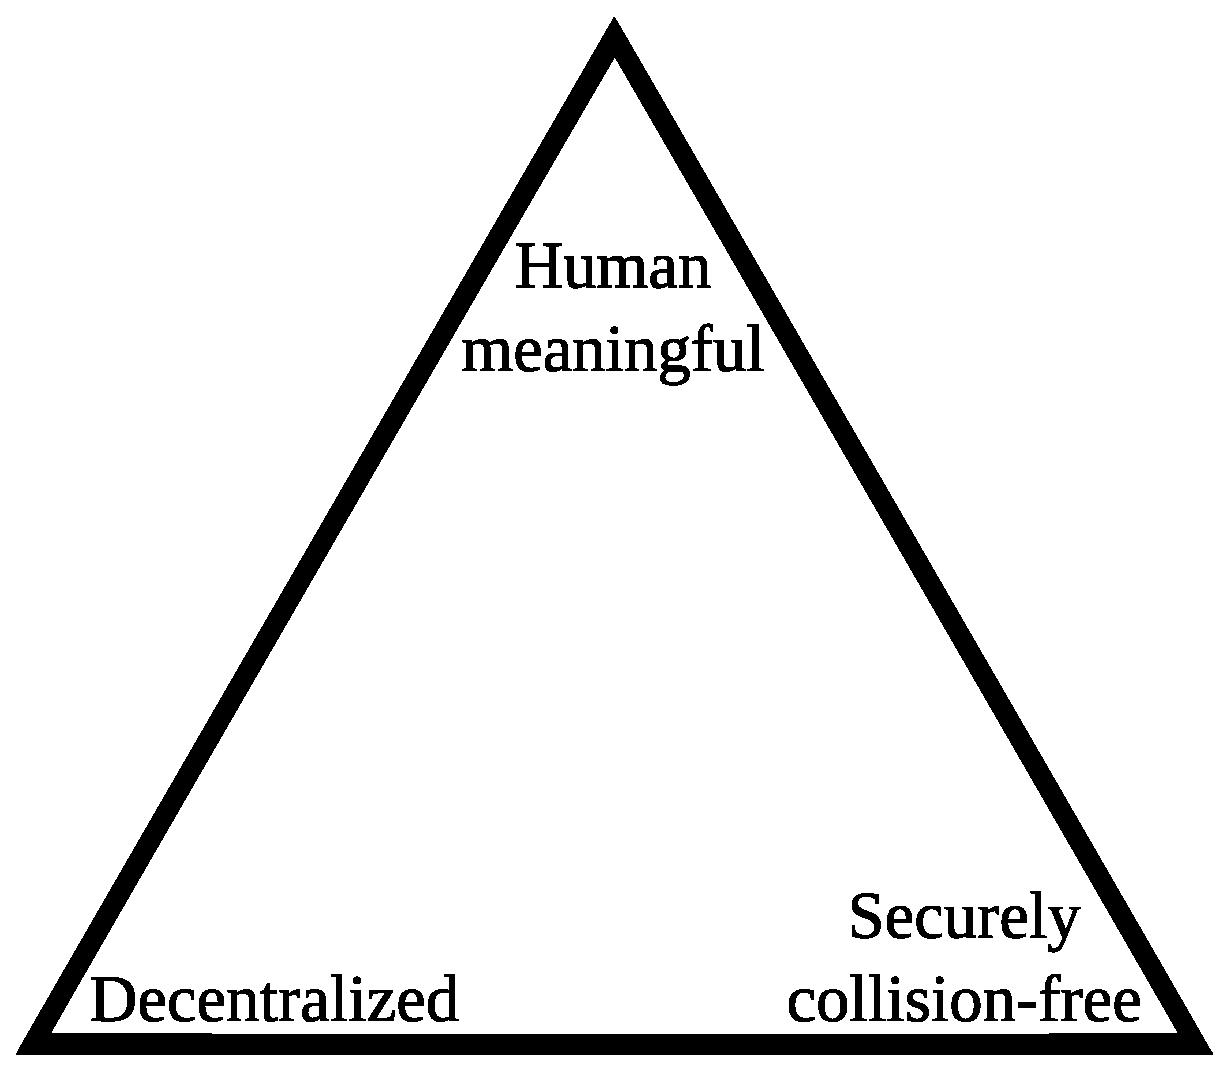
\includegraphics[width=0.3\textwidth]{../images/Zooko.eps}
	\caption{Zooko's Triangle.}
	\label{fig:figure8}
\end{figure}

For example, Tor hidden service .onion addresses and Bitcoin addresses are secure and decentralized but are not human-meaningful. Internet domain names are memorable and provably collision-free, but use central database managed DNS under the jurisdiction of ICANN. Finally, human nicknames are meaningful and distributed, but not securely collision-free.\cite{Stiegler2005}

In recent years, systems have been developed that have shown Zooko's Triangle to be false. One prominent example is Namecoin, a naming system which uses a Bitcoin-like blockchain to store name-value pairs. Human-meaningful names can be embedded in the blockchain, which is distributed by nature. The uniqueness of the names is ensured by the Namecoin network and can be verified with anyone holding the blockchain. However, Tor developers have been wary of using Namecoin to store domain names for Tor hidden services. It is also impractical to require all Tor clients to download the entire blockchain before being able to use a hidden service DNS system, and there are inherent security challenges involved with querying servers or the Namecoin network for a registration without being able to use a complete blockchain to verify it. Therefore, another solution is needed.

\section{Design Principles}

A high degree of anonymity, privacy, and security are of paramount importance for all Tor users. This context makes the inclusion of additional capabilities challenging. To meet these challenges and to remain acceptably resistant to attack, any proposed DNS system for Tor hidden services must meet at least the following requirements:

\begin{enumerate}
	\item The registrations must be anonymous; it should be infeasible to identify the registrant from the registration, including over the wire.
	\item Lookups must be anonymous; clients must stay anonymous when looking up registrations, otherwise they leak what hidden services they are interested in.
	\item Registrations must be publicly confirmable; akin to SSL certificates on the clearnet, clients must be able to verify that the registration matches and came from the service they are after, and is not a forgery.
	\item Registrations must be securely unique, or have an extremely high chance of being securely unique such as when this property relies on the collision-free property of cryptographic hashes.
	\item It must be distributed. The Tor community will adamantly reject any centralized solution for Tor hidden services for security reasons, as they have in the past for other proposals.
	\item It must remain simple to use. Most Tor users are not security experts and Tor puts almost all cryptographic details and routing details behind the scenes.
	\item It must remain backwards compatible; the existing Tor infrastructure must still remain functional.
	\item It should not be possible to maliciously modify or falsify registrations in the database or in transit, even though insider attacks.
\end{enumerate}

The current Tor hidden service protocol meets these requirements, but does not provide human-meaningful domain names so it suffers in usability. Existing literature proposing DNS systems for Tor is fairly sparse, though some ideas have been put forward. One of the most prominent is a 2011 Bachelor's thesis which outlines representing a hidden service's domain name as a series of words, rather than a base58-encoded hash.\cite{NicolussiThesis2011} However, while this scheme would improved recognition and memorability of hidden services, the words would remain random, are not chosen in advance, and do not relate to the hidden service in any meaningful way. Therefore this solution is an improvement but is not a solution. The problem remains open.

\section{Proposal}

I propose a new DNS system for Tor hidden services, which I am calling EsgalDNS. \textit{Esgal} is a Sindarin Elvish word from the works of J.R.R Tolkien, meaning "cloaked" or "hidden". EsgalDNS, as it stands currently, is a distributed DNS system embedded within the Tor network. At a high level, it is as follows: a domain registration, generated by the owner of a hidden service, is broadcasted across the Tor network. Every node votes as to whether or not this domain is already taken, according to that node's list of registered domains. The votes are then aggregated and broadcasted to all nodes. Since every node has the public keys of all other nodes, it can verify every votes. If a significant majority of the network vote that the domain is available, participating nodes then record that registration in their local storage. These lists are kept in synchronization. I build this system under the assumption that the majority of the Tor network is not actively malicious and will act honestly, which I consider a valid assumption considering that the security and usability of the Tor network would be entirely compromised if that assumption was shown to be false. Working under this assumption, I can obtain all three properties of Zooko's Triangle.

EsgalDNS, like other DNS systems, will support several commands, including Query, Create, Modify, Move, Renew, and Delete. In my thesis I will described and implement all six commands; however in this paper I will only address Query, a registration lookup, and Create, the generation of a new registration.

\subsection{Domain Registration}

A domain registration consists of eight components which are tied together by digital signatures and proof-of-work. The components are \textit{nonce}, \textit{authHash}, \textit{time}, \textit{domain}, \textit{subdomains}, \textit{contact}, \textit{digSig}, and \textit{pubKey}.

\begin{description}
	\item[nonce] \hfill \\
		An eight-byte number that serves as a source of randomness for the proof-of-work.
	\item[authHash] \hfill \\
		A 32-byte value containing the SHA256 hash of the digital signature on the consensus document published by the authority nodes. Consensus documents are generated frequently, so \textit{authHash} will be based on the document published at 00:00 GMT that day.
	\item[time] \hfill \\
		A four-byte integer holding the number of seconds since January 1st, 2013.
	\item[domain] \hfill \\
		A null-terminated cstring of the human-meaningful domain that will be correlated with the traditional .onion address of the hidden service. This can be up to 32 characters long. The TLD is .tor
	\item[subdomains] \hfill \\
		Up to 255 bytes of subdomain data, preceded by one byte that indicates the byte length. Each subdomain is null-terminated, so with the null characters 15 subdomains are possible when each is 16 characters long.
	\item[contact] \hfill \\
		16 bytes representing the last 32 base64-encoded bytes of the fingerprint of the service operator's PGP key, if they have one. If they do not, these bytes are zeroed. The purpose of this field is to allow the operator to be contacted securely.
	\item[digSig] \hfill \\
		The digital signature of all preceding fields.
	\item[pubKey] \hfill \\
		The public key of the hidden service.
\end{description}

To generate a registration, \textit{domain}, \textit{subdomains}, and \textit{contact} are determined by the operator, while \textit{authHash} and \textit{time} are filled in automatically. The hidden service operator then has to find a value for \textit{nonce} such that the proof-of-work is valid, specifically that that the SHA256 of \textit{digSig} is less than a target value \textit{T}. I plan to set \textit{T} such that the proof-of-works takes a significant amount of time on a modern CPU. This makes registering a domain expensive, thwarting flooding attacks. If \textit{nonce} is found, the registration is valid and ready for broadcast.

Two common proof-of-work systems are hashing, typically double-SHA256 ($ \textrm{SHA}256^{{2}} $) in the case of Bitcoin, and scrypt, a password-based key derivation function used by Litecoin. I chose the latter here; scrypt is a harder proof-of-work system because it requires large quantities of RAM in addition to CPU time, making brute-forcing significantly more challenging. Finding \textit{nonce} is made even more difficult because for every \textit{nonce}, a new digital signature must be made using the service's private key. This slows mining, complicates porting to GPUs and other specialized hardware, and prevents outsourcing to a outside computational resource. The digital signature ensures that all field are authenticated to the key of the hidden service, verifiable by all.

\subsection{Registration Broadcast}

Once a hidden service registration is complete and computationally valid, it is broadcasted to all nodes in the Tor network. However, Tor consists of approximately 6,100 relays, and broadcasting to them all directly is impractical; the broadcast is time-consuming, risks compromising the hidden service's location, and incurs a non-trivial load on the network. Therefore the network is broken into more practical sizes by delegate and subdelegate nodes, who forward the broadcast. The size of the delegate node set and size of the subdelegate node set are both equal to $ \floor*{\sqrt[3]{n}} = X $ where $ n $ is the number of nodes in the Tor network. With $ n $ currently equal to 6,100, $ X = 18 $, so the broadcast is sent to 18 delegate nodes, who each forward on to 18 subdelegate nodes, who then contact 18 other relays. This is far more practical.

The list of delegate and subdelegate nodes changes daily, but is known by all participants. A PRNG such as Mersenne Twister is seeded by \textit{authHash}. The PRNG then scrambles a numerical list of Tor nodes. The first $ X $ in the scrambled list are delegate nodes, the next $ X $ set of $ X $ nodes are the respective subdelegates. The remaining nodes are contacted by the subdelegates.

Each node then votes on the proposed registration. A vote consists of \textit{decision}, \textit{hash}, \textit{count}, \textit{root}, and \textit{signature} where \textit{decision} is either \textit{available}, \textit{unavailable}, or \textit{invalid}; \textit{hash} is the SHA256 of the registration it received; \textit{count} is the number of valid registrations it has in local storage; \textit{root} is the root node of the Merkle tree formed by those registrations; and \textit{signature} is the digital signature of the preceding fields. The vote are then aggregated, shared and combined among the delegates, and then send back down. Each node receives a copy of the votes from all nodes. If a significant majority vote \textit{available}, the node records the registration. The votes are then stored in a distributed hashtable in the Tor network so that they can be retrieved at a later date.

\textit{count} and \textit{root} will both be used to keep nodes synchronized with one another. Although I won't go into detail here, my plan calls for out-of-date nodes to attempt to synchronize with the node that advertises the highest \textit{count}. Synchronization also involves checking the votes, so falsely advertising a high \textit{count} isn't sufficient to mislead the network. \textit{root} is useful because it enables quick verification that nodes have synchronized lists and the use of a Merkle tree in general allows efficient synchronization when a node is out-of-date.

\subsection{Registration Query}

A client requesting \textit{example.tor} can anonymously query Tor nodes for any registration under that name. If it exists, it is returned and can be validated by the client's machine. The list of votes can optionally be retrieved if the client wishes to verify the secure uniqueness of that domain. The client can then extract \textit{pubKey} from the registration, hash it and truncate it, and look up the .onion in the traditional manner.

\section{Open Problems}

Some open problems that I need to address include:

\begin{enumerate}
	\item How frequently should domains expire? Are there any security risk in sending a Renew request?
	\item What minimum percentage of the network must vote? I need to know the percentage of the Tor network that is reachable at any given time.
	\item How many nodes in the Tor network should be assumed to be actively malicious? What are the implications of increasing this percentage?
	\item What attack vectors are there on the delegate and subdelegate nodes, and how can I thwart the attacks?
	\item What are the implications of a node intentionally voting the opposite way, or ignoring the request altogether?
	\item What other open problems are there?
\end{enumerate}

\section{Conclusion}

I have provided a brief and high-level overview of EsgalDNS, a distributed consensus-based DNS system inside the Tor network. The system provides a uniquely secure one-to-one mapping between human-meaningful domain names and traditional Tor .onion addresses. Registrations are publicly confirmable, so all involved parties can verify the authenticity, integrity, and uniqueness of the registration. Although this design is nowhere near finalized, I believe that my current setup is both promising and novel. I am planning experiments, testing in a simulation of the full Tor network, and of course more research. If accepted by the Tor community, I believe that EsgalDNS will be a valuable infrastructure that will significantly improve the usability and popularity of Tor hidden services.

\bibliographystyle{plain}
\bibliography{paper}

\end{document}
